\documentclass[]{article}
\usepackage[cm]{fullpage}
\usepackage{textcomp}
\usepackage{array}
\usepackage{sectsty}
\usepackage{amsmath}
\usepackage{amssymb}
\usepackage{amsfonts}
\usepackage{tipa}
\usepackage{verbatim}
\usepackage{multirow}
\usepackage{graphicx}
\newcommand{\mbb}[1]{$\mathbb{#1}$}
\newcommand{\tyen}{T\textyen}
\newcommand{\bb}[1]{\mathbb{#1}}
\newcommand{\bbs}[2]{$\mathbb{#1}_{#2}$}
\newcommand{\cst}[1]{$_{\text{#1}}$}
\newcommand{\normal}{\vartriangleleft}
\allsectionsfont{\mdseries\itshape}
\graphicspath{{/},{/cardfile/JPEGs/}}

%opening
\title{ZAIBATSU}
%\author{Jacob Kopczynski}
\date{}

\begin{document}
\maketitle

\section*{Overview}

\textbf{Zaibatsu} is a game of corporate competition in an ugly free market world, for 2-4 players (best with 3). Each player represents a megacorporation (\textit{Zaibatsu} in Japanese) competing to buy out juicy smaller companies and assemble the most powerful conglomerate to dominate the world economy. You and your fellow players will divide up the whole economy between you; ensure you get the most expansive, most self-sufficient organization out of the deal, and the economy will bend to the will of your \emph{Zaibatsu}.

\subsection*{Goal}

The winner will be the player with the highest total score at the end of the game. Points are scored for each company which is supplied with the resources it needs to operate. Companies which need more complex resources will score more points if properly supplied, so you will be well rewarded for stringing together full supply chains from the basic 1-point companies which produce raw materials up to the largest 10-point companies which assemble complex end products.

\subsection*{Contents}

\begin{itemize}
\item 48 Company Cards (21 mining companies, 22 processing companies, and 5 manufacturing companies)
\item 5 numbered auction cards
\item 1 Commissioner card
%\item Money chips; 20 green \tyen 1 pieces and 20 blue \tyen 5 pieces
\item Resource chits (24 each of red, yellow, and green, 7 each of orange and black, 5 each of white and blue, and 20 brown)
\end{itemize}

\section*{Setup}

Several aspects of setup and the beginning of the round depend on the number of players. Set out one more auction marker than there are players in the game in the center of the table and select a starting player to be given the Commissioner marker. This should be the player who has most recently purchased something made in Japan. If there is a disagreement or confusion, or the players consider this unfair, determine the first Commissioner randomly instead.
\ \\
Then give each player starting money and deal their cards for the first round, as shown in the chart below. One \tyen \ is 1 trillion Japanese yen (about \$10 billion), and is the smallest unit of currency that may be bid.

\begin{tabular}{ll|l|l|l|l|}
\cline{2-6}
\multicolumn{1}{l|}{} & \multirow{2}{1.7cm}{Cards per Player} & \multicolumn{4}{c|}{Starting Money for Each Player} \\
\cline{1-1} \cline{3-6}
\multicolumn{1}{|l||}{Players} & & 1st & 2nd & 3rd & 4th \\
\hline
\multicolumn{1}{|l||}{2} & 6 & \tyen 9 & \tyen 10  & &\\
\multicolumn{1}{|l||}{3} & 4 & \tyen 8 & \tyen 9 & \tyen 10 & \\
\multicolumn{1}{|l||}{4} & 3 & \tyen 9 & \tyen 9 & \tyen 10  & \tyen 10 \\
\hline
\end{tabular}

\section*{Understanding Company Cards}

Company cards have three parts; a score, written in the bottom left corner of each card, the input resources, and the output resources. These resources are laid out along the long top edge of the card, with an arrow pointing to the right separating them; input resources lie to the left of the arrow, output resources to the right.

\begin{figure}[h]
\end{figure}
There are 7 resource types: The 3 basic resources are red diamonds, yellow half-circles, and green squares. The intermediate resources are orange Xs and black plus signs. The advanced resources are white hexagons and blue stars. Creating the higher levels of resource requires combining resources from lower levels. Additionally, not all combinations exist; no company uses red to produce black or uses green to produce orange, and no company uses orange to produce blue, or black to produce white. Yellow is a flexible resource, used in every type of processing but rarely used alone.

\begin{figure}[h]
\begin{minipage}{.4\textwidth}
  \centering
  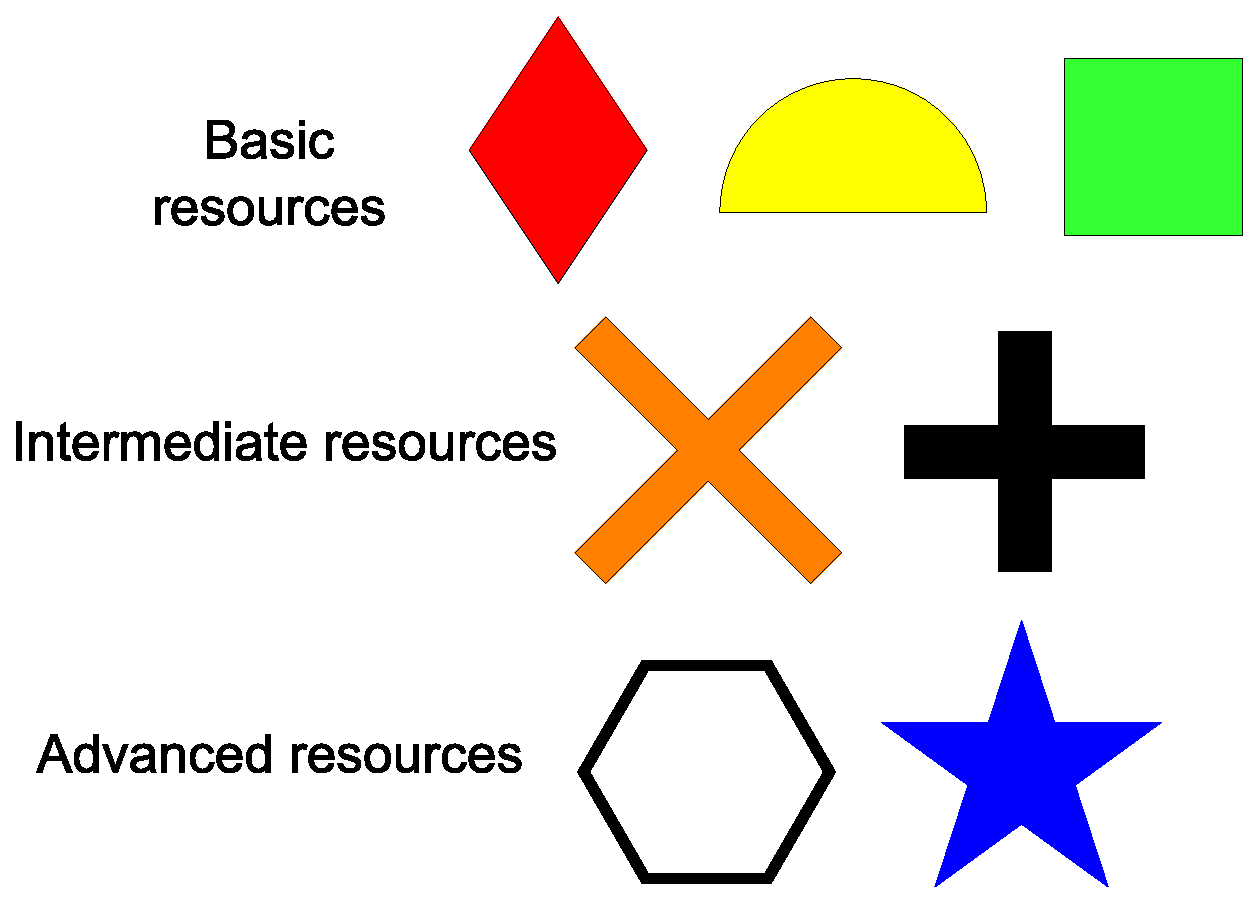
\includegraphics[scale=0.25]{cheatsheet}
  \label{fig:test1}
\end{minipage}%
\begin{minipage}{.3\textwidth}
  \centering
  \fbox{\includegraphics[scale=0.13,angle=-90]{mining}}
  Mining Company
  \label{fig:test2}
  \fbox{\includegraphics[scale=0.13,angle=-90]{processing1}}
  Simple Processing Company
\end{minipage}
\begin{minipage}{.3\textwidth}
  \centering
  \fbox{\includegraphics[scale=0.13,angle=-90]{processing2}}
  Complex Processing Company
  \label{fig:test2}
  \fbox{\includegraphics[scale=0.13,angle=-90]{manufacturing}}
  Manufacturing Company
\end{minipage}
\end{figure}
Companies come in three varieties; Mining companies produce raw materials and require no input resources to operate; they are marked 1 point each, which they always score, and produce basic resources. Processing companies have both input and output resources; if they are supplied with their input resources, they produce their outputs and score. These are split into two sub-types; some produce intermediate resources and score 2 points when operating, and other produce advanced resources and score 5 points when operating. The third kind of company is the manufacturing companies, which have inputs, but lack output resources. If they are operating, they produce 10 points each from the consumer goods they sell or government contracts they fulfill.

\begin{minipage}{.3\textwidth}
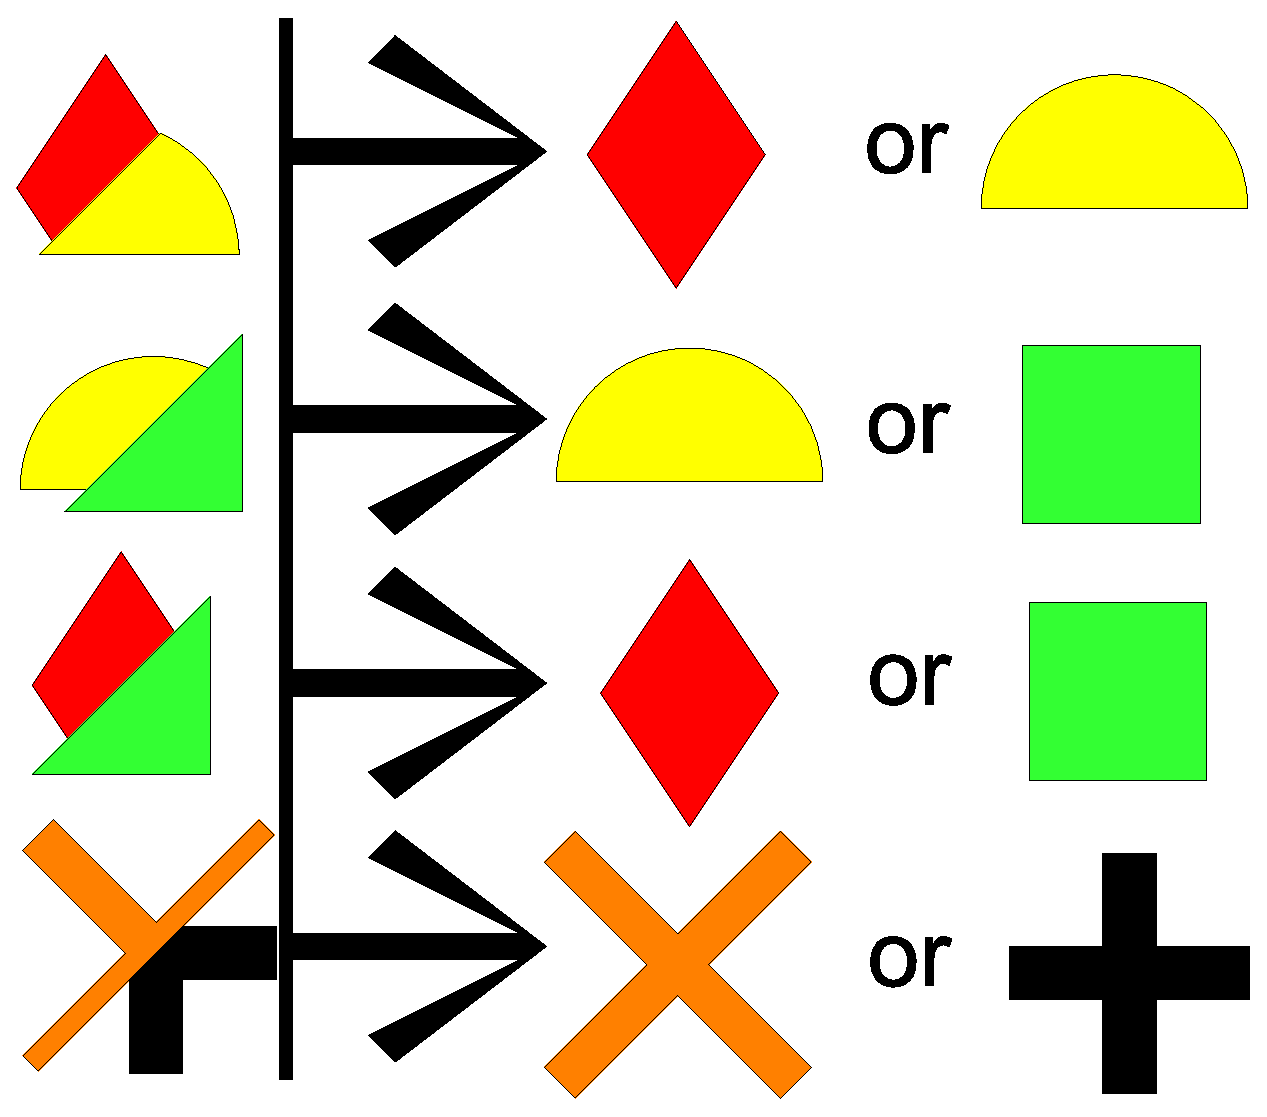
\includegraphics[scale=0.2]{hybrids}
\end{minipage}
\begin{minipage}{.7\textwidth}
Some companies have output resource symbols which are two different shapes and colors, split along a central diagonal line. Each of these symbols represents the capability to produce one resource of either type. Mining companies of this type all have two symbols; they may generate two of either type, or one of each. This decision is made independently for each company.
\end{minipage}



\pagebreak
\section*{The Round}

At the beginning of each round after the first, each player must receive new cards and money, and the Commissioner marker passes to the left. Give each player \tyen 10 from the bank, and deal 12 cards per round, split among the players evenly as shown in the table above. The round has two parts: first, the players will take turns placing the cards in their hands into auction piles, one card at a time. When all cards have been placed, the players will take turns calling the auctions and bid on them in turn.

\subsection*{The Deal}

Starting with the player with the Commissioner marker and proceeding to the left, players take turns placing one card at a time from their hands into the auctions. These cards may be placed into empty auctions or into auctions that already have several cards, and some auctions may end the deal empty. Auctions are limited to the number of auction markers in use this game, which is always one more than the number of players. Once every player's hand is empty, proceed to the auction.

\subsection*{The Auction}

Starting with the player with the Commissioner marker, players each take a turn to call an auction for bid. The player to their left bids first, and the auction-caller bids last. Auctions in \emph{Zaibatsu} are single-bid, proceed clockwise, and end with the player who selected the auction. The first bid may be any number of \tyen ; bids may not be 0, but a player may always pass. Further bids may either top the high bid, or pass. When the player who designated the auction has either bid or passed, the auction is over, and the high bidder wins the auction, paying their bid to the bank and taking all company cards in the auction pile into their conglomerate.

All piles will be auctioned; even an empty pile will be auctioned, though it is most likely that all players will pass. This means that the Commissioner for the round will call two auctions; the first one of the round, and the last. Once the final auction is completed, the round ends, all auction tiles are flipped back to face up, %and the next scoring phase or round will begin.
and the next round will begin. % currently writing this as though there isn't a mid-game scoring phase

\indent\textit{Example: Sumitomo is the Commissioner this round and calls the auction for a small pile. Mitsui, to their left, is not interested, and pass. Mistubishi bid \tyen 4 and Yasuda pass. Sumitomo bid \tyen 5 and take the pile, adding all its companies to their conglomerate. Mitsui picks another pile and begins the next auction; Mitsubishi bids first, and Mitsui will bid last.}

\subsection*{Your Conglomerate}

When a player wins an auction, all companies in the auction are included into that player's conglomerate. The conglomerate should be displayed on the table in front of them, face up. When acquiring companies, place resource cubes of the appropriate color on each mining company for each resource it creates; if there are flexible resources (those with a diagonal split) for which you have not made a decision, use brown cubes. These can be moved to processing and manufacturing companies as you are able to supply them; as processing companies are fully supplied, add the appropriate intermediate or advanced resource cubes on those cards. In this way, you can track what resources you have extra supply of, and what you most need.

\section*{Scoring}

%Points are scored twice in the game. Once after round 2, and then again at the end of the game, after round 4. 
When scoring, each player determines how many of the companies in their conglomerate can be properly supplied. Each company which can be supplied with the appropriate resources is \emph{operating} %for that scoring phase 
and will score and produce its own output resources. No company can operate more than once% in the same scoring phase
, even if your conglomerate produces enough resources to supply it fully two or more times. %If you have excess resources of some type, they will be wasted, and may not be kept for future scoring phases.
Tracking your progress with resource cubes should speed up this process greatly.

%\indent You may track your resources available and produced in any way you wish, but new players or players with particularly complex conglomerates may want to track them using the resource cubes. These cubes come in all the colors of resources (red, yellow, green, orange, black, white, and blue), as well as brown cubes which can represent split resources for which you have not yet made a decision. We recommend placing all cubes produced by the mining companies, then moving them to your processing companies as you determine which companies you will supply and adding appropriately-color cubes on those processing companies as they become fully supplied. These output cubes then can be moved to further processing companies and manufacturing companies as needed, while the input cubes remain on the company. This allows you to quickly track which companies are operating (those which have all their inputs) and, if you change your mind about the best way to allocate resources, allows you to backtrack easily.

When you are satisfied that you have run your conglomerate as well as possible, count up the score of each company which is operating, and %report the sum of those values as your score for the phase. When all players have completed this process, proceed to the next round, or to end of the game if the final round was already finished.
%#SPECIFIC TO NO-MIDDLE-SCORING VERSION
add 1 point for each 3\tyen you have remaining. The highest total score is the most dominant zaibatsu and is in control of the economy for the next generation. If two players are tied, they share control; everyone else is out of luck.

%\subsection*{End of the Game}

%The two scoring phases are counted separately, and at the end of the game those two scores are added together. Each player also scores extra points from their remaining money; score one additional point per \tyen 3. The player with the highest score is the most dominant zaibatsu and is in control of the economy for the next generation. If two players are tied, they share control; everyone else is out of luck.

%\indent Note: In the event of an apparent tie, fractional scores should be calculated, so every \tyen\ can make a difference.
%#DESIGN NOTE: I think this should be removed. Ties are rare anyway.

\end{document}
